\documentclass[11pt]{article}
\usepackage{tikz}
\usetikzlibrary{shadows,arrows,positioning}
% Define the layers to draw the diagram
\pgfdeclarelayer{background}
\pgfdeclarelayer{foreground}
\pgfsetlayers{background,main,foreground}

% Define block styles
\tikzstyle{materia}=[draw, fill=blue!20, text width=6.0em, text centered,
  minimum height=1.5em,drop shadow]
\tikzstyle{etape} = [materia, text width=8em, minimum width=10em,
  minimum height=3em, rounded corners, drop shadow]
\tikzstyle{texto} = [above, text width=6em, text centered]
\tikzstyle{linepart} = [draw, thick, color=black!50, -latex', dashed]
\tikzstyle{line} = [draw, thick, color=black!50, -latex']
\tikzstyle{ur}=[draw, text centered, minimum height=0.01em]

% Define distances for bordering
\newcommand{\blockdist}{1.3}
\newcommand{\edgedist}{1.5}

\newcommand{\etape}[2]{node (p#1) [etape]
  {#2}}

% Draw background
\newcommand{\background}[5]{%
  \begin{pgfonlayer}{background}
    % Left-top corner of the background rectangle
    \path (#1.west |- #2.north)+(-0.5,0.25) node (a1) {};
    % Right-bottom corner of the background rectanle
    \path (#3.east |- #4.south)+(+0.5,-0.25) node (a2) {};
    % Draw the background
    \path[fill=yellow!20,rounded corners, draw=black!50, dashed]
      (a1) rectangle (a2);
      \path (#3.east |- #2.north)+(0,0.25)--(#1.west |- #2.north) node[midway] (#5-n) {};
      \path (#3.east |- #2.south)+(0,-0.35)--(#1.west |- #2.south) node[midway] (#5-s) {};
      \path (#3.east |- #2.north)+(0.7,0)--(#3.east |- #4.south) node[midway] (#5-w) {};
  \end{pgfonlayer}}

\newcommand{\transreceptor}[3]{%
  \path [linepart] (#1.east) -- node [above]
    {\scriptsize #2} (#3);}

\begin{document}
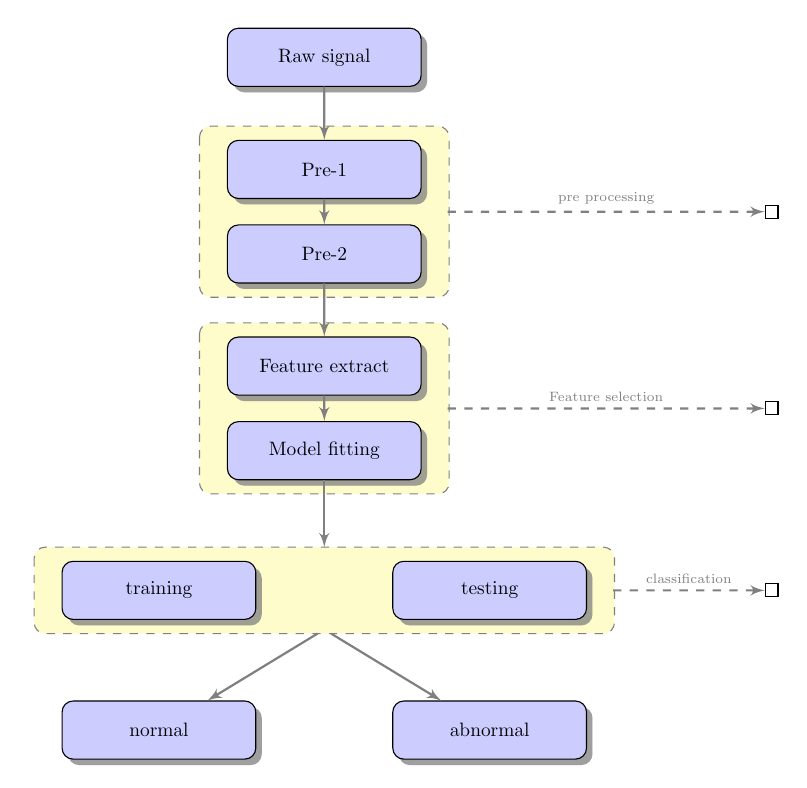
\begin{tikzpicture}[scale=0.7,transform shape]

  % Draw diagram elements
  \path \etape{1}{Raw signal};

  \path (p1.south)+(0.0,-1.5) \etape{2}{Pre-1};
  \path (p2.south)+(0.0,-1.0) \etape{3}{Pre-2};

  \path (p3.south)+(0.0,-1.5) \etape{4}{Feature extract};
  \path (p4.south)+(0.0,-1.0) \etape{5}{Model fitting};

  \path (p5.south)+(-3.0,-2.0) \etape{6}{training};
  \path (p5.south)+(3.0,-2.0) \etape{7}{testing};
  \node [below=of p5] (p6-7) {};

  \path (p6.south)+(0.0,-2.0) \etape{8}{normal};
  \path (p7.south)+(0.0,-2.0) \etape{9}{abnormal};
  \node [below=of p6-7] (p8-9) {};

  % Draw arrows between elements
  \path [line] (p1.south) -- node [above] {} (p2);
  \path [line] (p2.south) -- node [above] {} (p3);
  \path [line] (p3.south) -- node [above] {} (p4);
  \path [line] (p4.south) -- node [above] {} (p5);

  \background{p2}{p2}{p3}{p3}{bk1}
  \background{p4}{p4}{p5}{p5}{bk2}
  \background{p6}{p6}{p7}{p7}{bk3}

  \path [line] (p5.south) -- node [above] {} (bk3-n);
  \path [line] (bk3-s) -- node [above] {} (p8);
  \path [line] (bk3-s) -- node [above] {} (p9);
  \path (bk1-w)+(+6.0,0) node (ur1)[ur] {};
  \path (bk2-w)+(+6.0,0) node (ur2)[ur] {};
  \path (bk3-w)+(+3.0,0) node (ur3)[ur] {};
  \transreceptor{bk1-w}{pre processing}{ur1};
  \transreceptor{bk2-w}{Feature selection}{ur2};
  \transreceptor{bk3-w}{classification}{ur3};
\end{tikzpicture}
\end{document}
